\section{Cross-site Scripting (XSS)}
The objective of a XSS attack is to inject malicious js into the victim's page. The attacker uses vulnerabilities in the web application, not the web browser, to execute malicious javascript code without the user's interaction. Malicious js can be very dangerous, as it can steal unprotected cookies, make requests in the user's behalf and modify the page's html to create phishing attacks, between many others. If an attacker can use the web app to execute js in another user's browser, the security of the site and it's users is severely compromised.

\subsection{Types of XSS}
There are several classifications for XSS types. The latest proposes a clear differentiation by the origin of the vulnerability.

\begin{itemize}
  \item \textbf{Back-end XSS} If the XSS occurs when the server sends HTML with malicious code injected in it by an attacker, we'll classify it as Server XSS or Back-end XSS
  \item \textbf{Front-end XSS} When the injection occurs on the DOM (Document Object Model, the interface presented by the browser to interact with the HTML in the page) we'll classify the vulnerability as a Client XSS or Front-end XSS
\end{itemize}

Also, inside each of these categories (front-end, back-end) we can differentiate by these two types

\begin{itemize}
  \item \textbf{Stored or Persistent XSS} Persistent XSS occurs when the attacker inserts the payload in a persistent database in the application (usually in the back-end, but can also be in the front-end in a HTML5 local storage.). This type of attack affects all the users that request the affected content and is considered the most dangerous.
  
  \item \textbf{Reflected XSS} Reflected XSS happens when the user input is returned immediately (search query, form, etc) and the input is not protected. This usually requires some sort of social engineering attack to be effective (tricking the victim to click a URL with malicious GET parameters, suggesting the victim to introduce a payload in a form ...)
\end{itemize}

\begin{table}[htb]
  \centering
  \caption{Classification table for XSS}
  \label{xss-table}
  \begin{tabular}{cllll}
    \cline{2-3}
    \multicolumn{1}{c|}{\textbf{XSS}}        & \multicolumn{1}{c|}{\textbf{Back-end}}      & \multicolumn{1}{c|}{\textbf{Front-end}}      &  &  \\ \cline{1-3}
    \multicolumn{1}{|c|}{\textbf{Stored}}    & \multicolumn{1}{l|}{Stored Back-end XSS}    & \multicolumn{1}{l|}{Stored Front-end XSS}    &  &  \\ \cline{1-3}
    \multicolumn{1}{|c|}{\textbf{Reflected}} & \multicolumn{1}{l|}{Reflected Back-end XSS} & \multicolumn{1}{l|}{Reflected Front-end XSS} &  &  \\ \cline{1-3}
    \multicolumn{1}{l}{}                     &                                             &                                              &  & 
  \end{tabular}
\end{table}
This classification can be summarized on the table \ref{xss-table}. The former definition included type called DOM-based XSS, that would now fall into the current Reflected front-end XSS.
Now we'll deeper explain two of the most usual kinds of XSS, Back-end Persistent XSS and Back-end Reflected XSS

\subsubsection{Back-end Persistent XSS}
In this attack, the malicious js is stored in the DB. The attacker can upload this js disguised in a comment of a post, a form, etc. The web app saves this code in the DB, and when the page is solicited by another user the code is inserted in the html unknowingly by the application. This is one of the most dangerous XSS, as any user who visits the site can be affected.

\begin{figure}[htb]
  \begin{centering}
    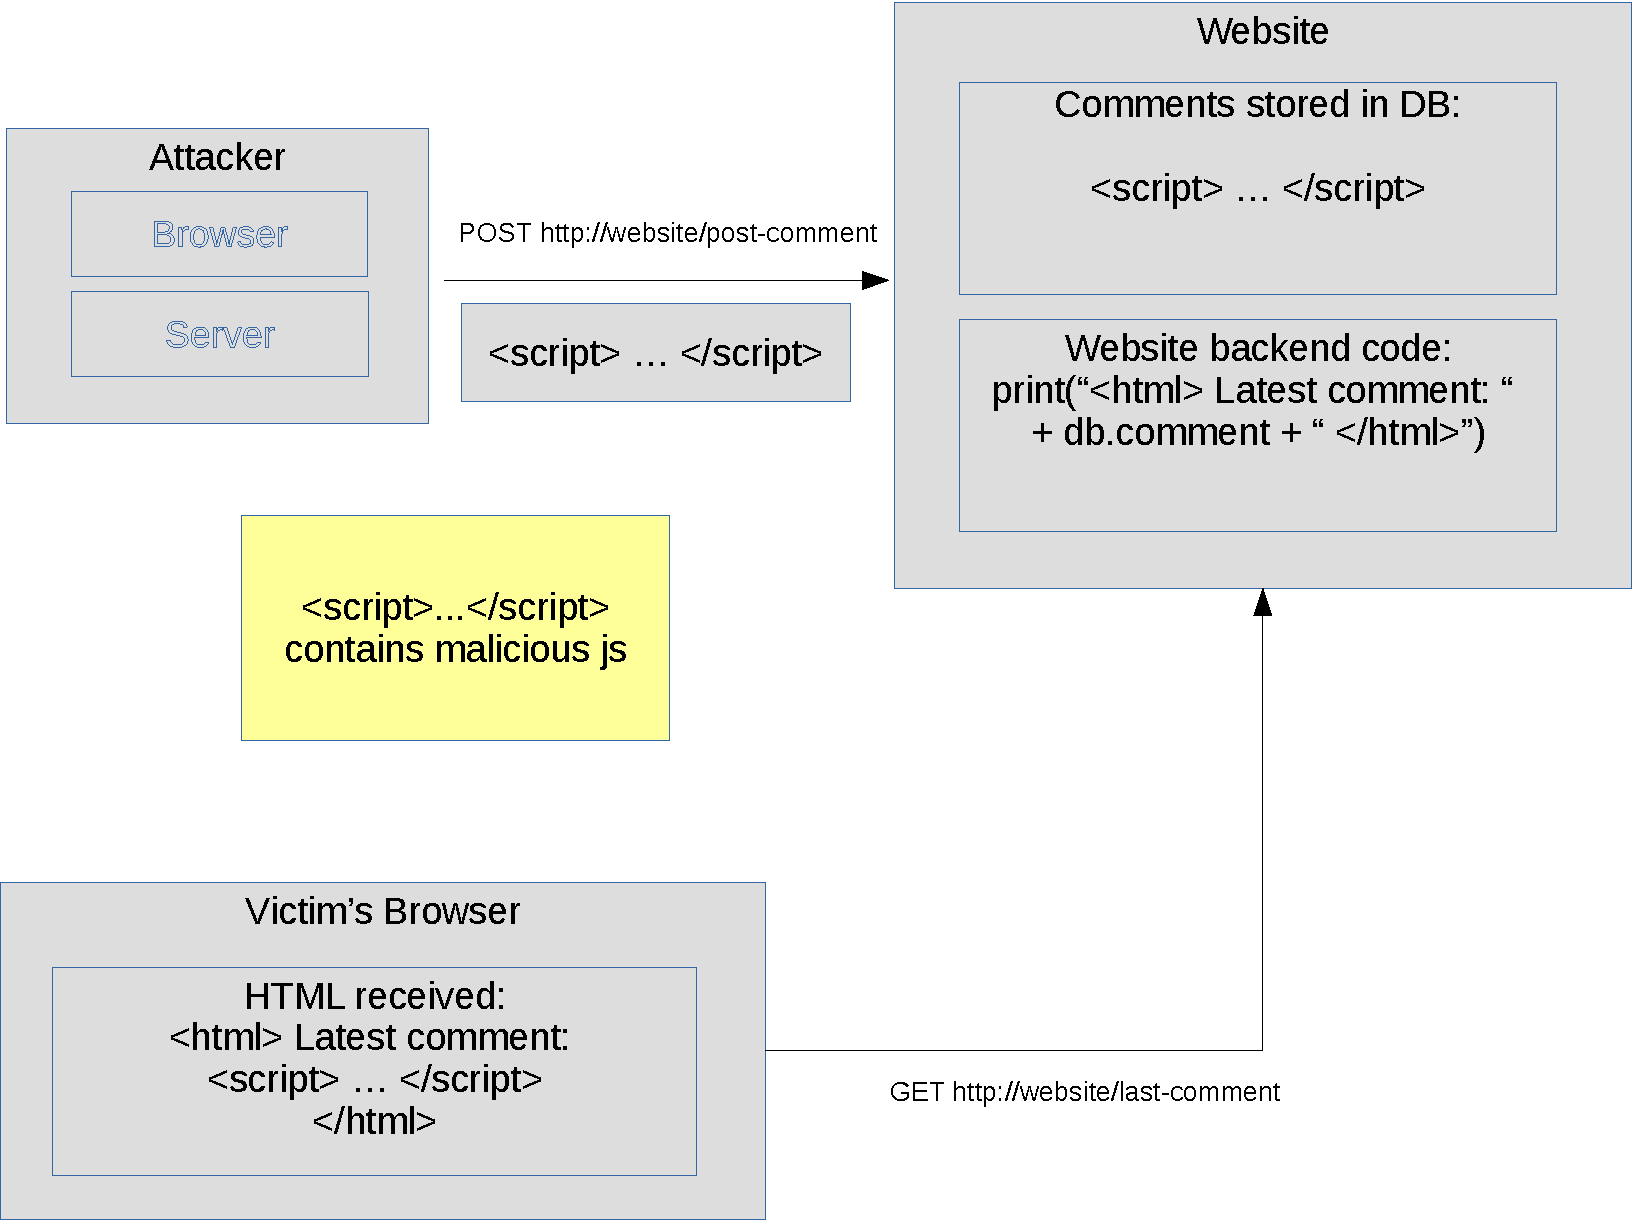
\includegraphics[width=0.7\columnwidth]{\securitydir/WebSec/figures/persistent-xss}
    \par\end{centering}
  \caption{\label{fig:persistent-xss} Diagram of a stored XSS exploit.}
\end{figure}

As shown on the figure \ref{fig:persistent-xss} these are the detailed steps involved in the process
\begin{enumerate}
  \item This website offers a comment section for the users to leave their opinion. The attacker posts a comment that contains malicious javascript code between script tags.
  \item The comment containing the payload gets as is into the web application's database.
  \item An unsuspecting user browsing the site requests the page where the comments are displayed.
  \item The website gets the comments from the database, inserts them to the page HTML and then sends the response to the victim.
  \item The victim's browser loads the HTML from the response received. Since the HTML contains a valid javascript code between script tags, the malicious javascript is executed.
\end{enumerate}


\subsubsection{Back-end Reflected XSS}
Reflected XSS usually require some kind of social engineering to make the user trigger the exploit. In this example the attacker needs to craft a malicious URL with js in it as a parameter. This is usually exploited passing a URL with a search query with the js as the paramater to search. The attacker then tricks the victim to open the link, generating a GET request and returning HTML page with the query inserted in it.

\begin{figure}[htb]
	\begin{centering}
		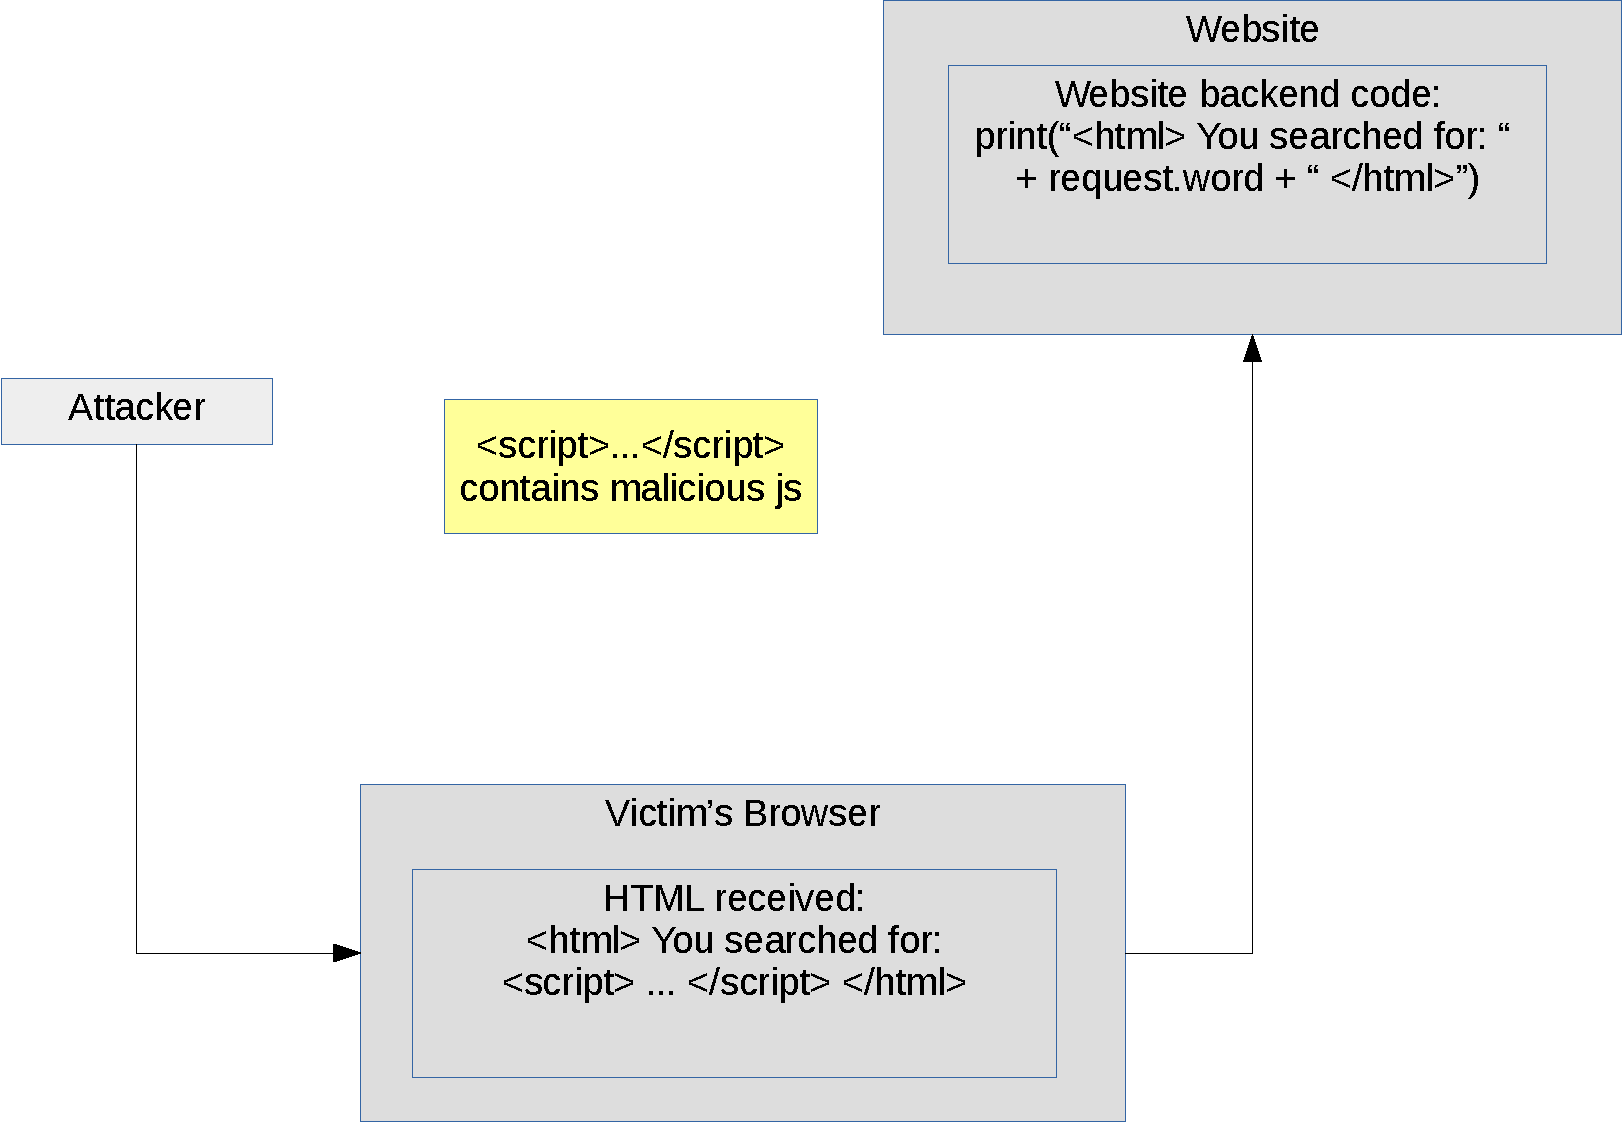
\includegraphics[width=0.7\columnwidth]{\securitydir/WebSec/figures/reflected-xss}
		\par\end{centering}
	\caption{\label{fig:reflected-xss} Diagram of a reflected XSS exploit.}
\end{figure}

As seen on figure \ref{fig:reflected-xss} the process is as follows:
\begin{enumerate}
  \item The attacker knows that the search function takes the words to search as a GET parameter in the GET request and crafts a URL that contains the malicious JS in the GET parameters. The attacker sends this URL to the victim with a misleading context in order to make the victim access it.
  \item The victim falls for the trick and requests the URL.
  \item The back end gets the GET parameter and searches its database for it. The search results are irrelevant, but the site prints a message in the response HTML with the searched word and that is where the malicious javascript gets inserted.
  \item The victim's browser gets the response with the malicious javascript inserted and it gets executed by the browser.
\end{enumerate}

\subsubsection{Front-end XSS (DOM-based XSS)}
In a Front-end XSS, the malicious javascript is inserted in the DOM by the front-end of the web application, and not by the server. The server does not have any kind of visibility to what is happening on the front end, as in this case the back-end only sends the HTML to the browser, and nothing else. This also means that the malicious javascript can come from other sources that are not visible to the server, like local storage, Indexed DB (in a Front-end Persistent XSS) or in a URL's fragment identifier (in a Front-end Reflected XSS).
